%%%%%%%%%%%%%%%%%%%%%%%%%%%%%%%%%%%%%%%%%%%%%%%%%%%%%%%%%%%%%%%%%%%%%%%%%%%%%%%%%%%
%%                 PŘÍLOHA - UŽIVATELSKÁ PŘÍRUČKA                                %%
%%%%%%%%%%%%%%%%%%%%%%%%%%%%%%%%%%%%%%%%%%%%%%%%%%%%%%%%%%%%%%%%%%%%%%%%%%%%%%%%%%%
\chapter{User guide}
\label{user-guide}

GIS.lab web console is as an application for management of GIS.lab
users and roles. It consists of two sections - user console
(\ref{user-console}) and admin console (\ref{admin-console}). Data are
synchronized between \zk{LDAP} server and local Django database. It is
currently available only as a Django project in virtual environment of
GIS.lab Desktop. Before installation of web console, please connect to
your existing GIS.lab server or install it on the basis of this
instruction:
\href{https://gislab.readthedocs.io/en/latest/installation/index.html}{https://gislab.readthedocs.io/en/latest/installation/\linebreak
  index.html}.

\section{Installation}
\label{installation}
%TK: nevím, jestli installation je vhodné slovo?

\begin{enumerate}
\item{Download script called \textsf{setup\_script.sh} from repository
  \href{https://github.com/ctu-geoforall-lab-projects/dp-kulovana-2019}{https://github.com/ctu-geoforall-lab-projects/dp-kulovana-2019}
  to your GIS.lab server.}

\item{Go to the directory where the script is located.}

\item{Open the script and assign the variable \textsf{PROJ\_PATH} to a
  full pathname of a directory where you want the web console project
  to be located \linebreak
  (e.g. \textsf{PROJ\_PATH=/mnt/home/gislab/web\_console}).}

\item{Run command:}
\begin{center}
\textsf{./setup\_script.sh}
\end{center}

\item{Go to the project directory
  (e.g. \textsf{/mnt/home/gislab/web\_console}), open file
  \textsf{web\_console\_project/settings\_custom.py} and assign the
  variable \linebreak\textsf{ALLOWED\_HOSTS} to your GIS.lab server
  \zk{URL}.}

\item{Activate virtual environment by running command:}
\begin{center}
\textsf{source virenv/bin/activate}
\end{center}

\item{Sync your existing \zk{LDAP} users and groups to Django database
  by running:}
\begin{center}
\textsf{manage.py ldap\_sync\_users}
\end{center}

\newpage
\item{Start up the server with:}
\begin{center}
\textsf{python manage.py runserver 0:8080}
\end{center}

\item{Go to the homepage at \textsf{ALLOWED\_HOSTS:8080} where
  \textsf{ALLOWED\_HOSTS} stands for assigned \zk{URL}.}

\item{Stop server with:}
\begin{center}
\textsf{CTRL+C}
\end{center}

\item{Deactivate virtual environment by running command:}
\begin{center}
\textsf{deactivate}
\end{center}
\end{enumerate}

\section{User console}
\label{user-console}

There is a user console available on the homepage
(e.g. http://b802-01.fsv.cvut.cz:8080). Its objective is to allow
users to registrate and to edit their personal information.

As a non-authenticated user, you see two buttons which redirect you to
either login page or a registration.
\begin{figure}[H] \centering
    
\includegraphics[width=430pt]{./prilohy/guide-user-home-unknown.png}
    \caption[User console - home page]{User console - home page (zdroj:
	\href{}{Tereza Kulovaná})}
	\label{fig:guide-user-home-unknown.png}
\end{figure}

\newpage
\textit{Username, first name, last name, email address} and
\textit{password} are mandatory fields for successful registration,
\textit{description} is optional. For sign up push the \textsf{SIGN
  UP} button. If the form is not valid, the error, with information of
what went wrong, shows. In case of a successful validation, you are
redirected to login page.
\begin{figure}[H] \centering
    
\includegraphics[width=430pt]{./prilohy/guide-user-user-add.png}
    \caption[User console - registration]{User console - registration (zdroj:
	\href{}{Tereza Kulovaná})}
	\label{fig:guide-user-user-add}
\end{figure}

\newpage
On login page you need to fill in your credentials. After successful
authentication, you are redirected to the page with your personal
information.
\begin{figure}[H] \centering
    
\includegraphics[width=430pt]{./prilohy/guide-user-login.png}
    \caption[User console - login page]{User console - login page (zdroj:
	\href{}{Tereza Kulovaná})}
	\label{fig:guide-user-login}
\end{figure}

For authenticated user, homepage displays their personal details and
active roles. \textsf{Edit} button allows you to change your personal
details.
\begin{figure}[H] \centering
    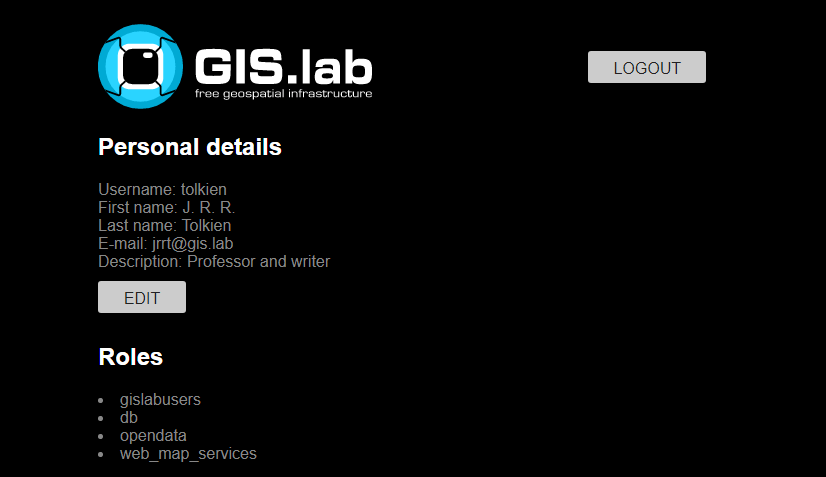
\includegraphics[width=430pt]{./prilohy/guide-user-home-known.png}
    \caption[User console - home page (authenticated user)]{User console - home page (authenticated user) (zdroj:
	\href{}{Tereza Kulovaná})}
	\label{fig:guide-user-home-known}
\end{figure}

From all of your atributes, you are not allowed to change
\textsf{username} field. For changing password, you need to click on
\textsf{this form} link in the text and you will be redirected to the
correct page.
\begin{figure}[H] \centering
    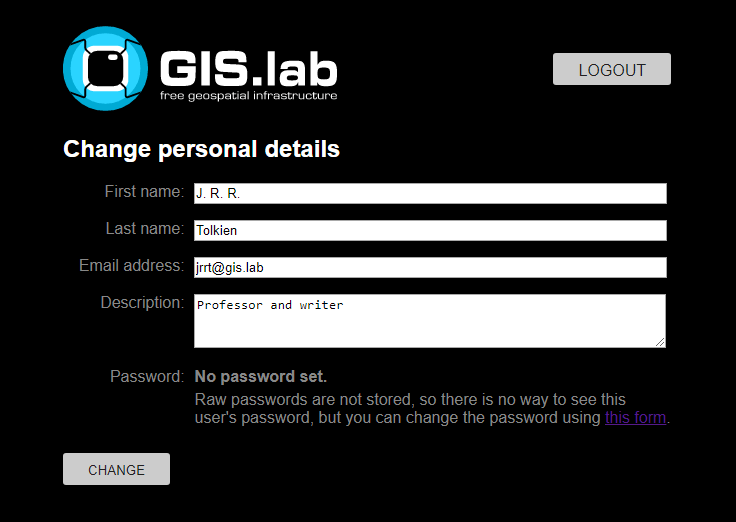
\includegraphics[width=430pt]{./prilohy/guide-user-change.png}
    \caption[User console - edit personal details]{User console - edit personal details (zdroj:
	\href{}{Tereza Kulovaná})}
	\label{fig:guide-user-change}
\end{figure}

Write your password twice for verification and push the
\textsf{CHANGE} button. In case of a successful change, your
credentials are updated and you are redirected to the homepage.
\begin{figure}[H] \centering
    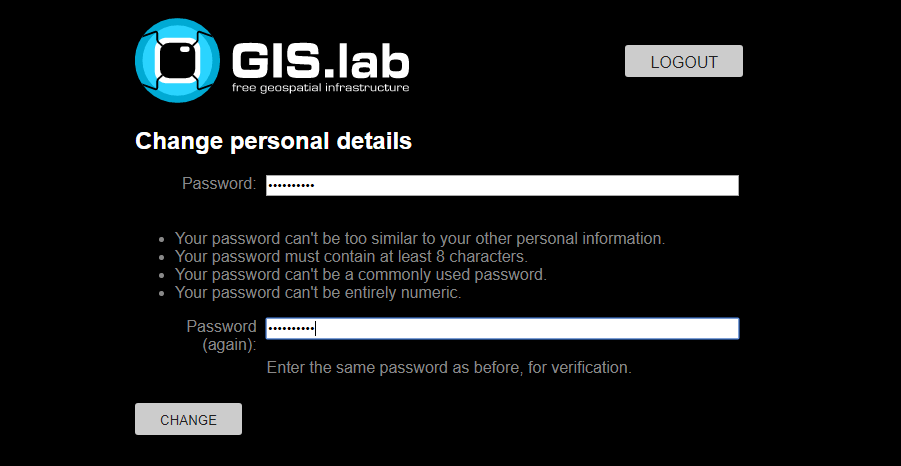
\includegraphics[width=430pt]{./prilohy/guide-user-password.png}
    \caption[User console - password change]{User console - password change (zdroj:
	\href{}{Tereza Kulovaná})}
	\label{fig:guide-user-password}
\end{figure}

Logout is available by \textsf{LOGOUT} button in the upper right
corner.

\section{Admin console}
\label{admin-console}

To access the admin console, you need to write \textit{/admin} behind
your homepage \zk{URL}
(e.g. http://b802-01.fsv.cvut.cz:8080/admin). Fill in your credentials
to log in to the admin console.
\begin{figure}[H] \centering
    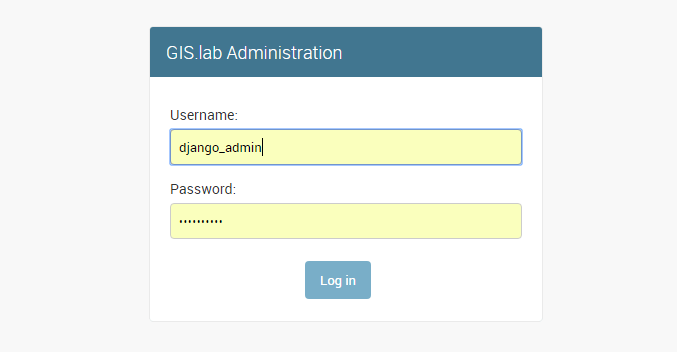
\includegraphics[width=430pt]{./prilohy/guide-admin-home-unknown.png}
    \caption[Admin console - login page]{Admin console - login page (zdroj:
	\href{}{Tereza Kulovaná})}
	\label{fig:guide-admin-home-unknown}
\end{figure}

There is a list of recent actions on the welcome page of GIS.lab
administration, as well as links to the list of users and the list of
groups (roles).
\begin{figure}[H] \centering
    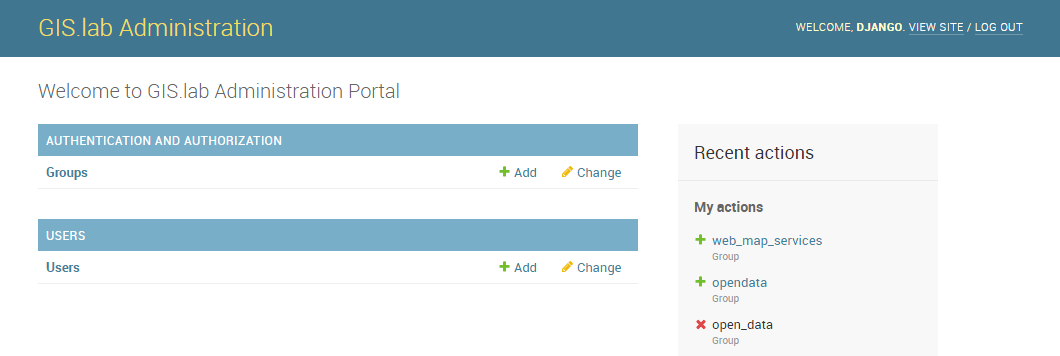
\includegraphics[width=430pt]{./prilohy/guide-admin-home-known.png}
    \caption[Admin console - home page]{Admin console - home page (zdroj:
	\href{}{Tereza Kulovaná})}
	\label{fig:guide-admin-home-known}
\end{figure}

User list displays all users in database and their \textit{username,
  first and last name, email address, description} and
\textit{superuser status}. You can filter users by superuser status or
by group membership. New user can be added by \textsf{ADD USER} button
in the upper right corner. You can change group membership and
personal details of a user by clicking on their username. If you want
to delete user, click on their username as well.
\begin{figure}[H] \centering
    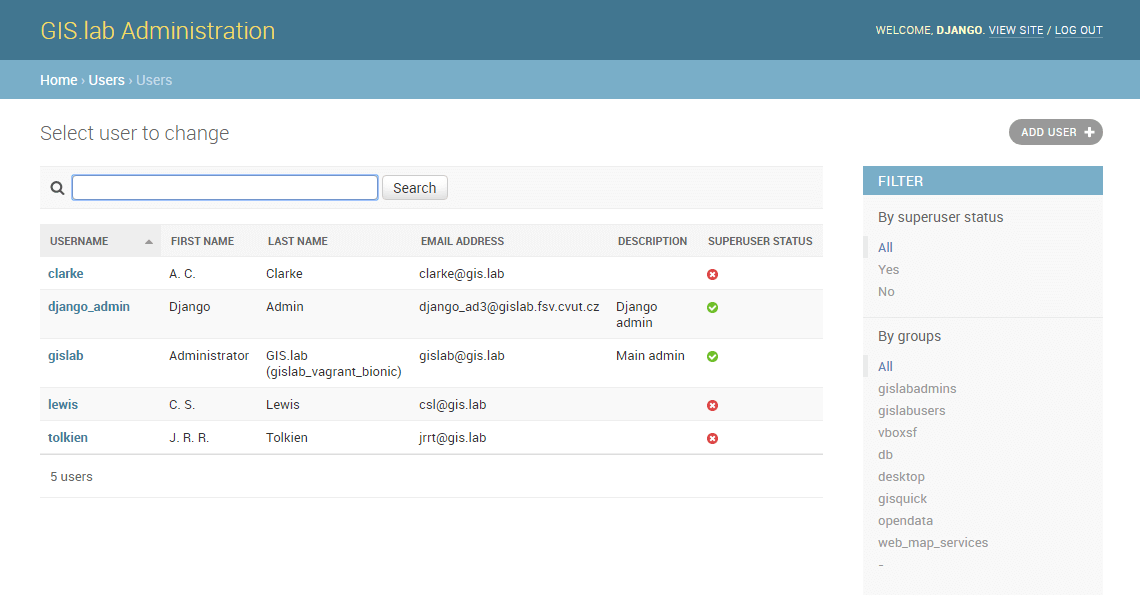
\includegraphics[width=430pt]{./prilohy/guide-admin-users.png}
    \caption[Admin console - users]{Admin console - users (zdroj:
	\href{}{Tereza Kulovaná})}
	\label{fig:guide-admin-users}
\end{figure}

On user details page you can change user's personal info or group
memberships. For changing password, you need to click on \textsf{this
  form} link in the text and you will be redirected to correct
page. To move groups between \textsf{Available groups} and
\textsf{Chosen groups}, highlight selected group(s) and click on
right/left arrow. You can move all groups in the same time by clicking
\textsf{Choose all/Remove all}. Push \textsf{SAVE} button in the
bottom right corner to reflect the changes.

You can delete user from database by pushing \textsf{Delete} button in
the bottom left corner. The decision has to be confirmed.
\begin{figure}[H] \centering
    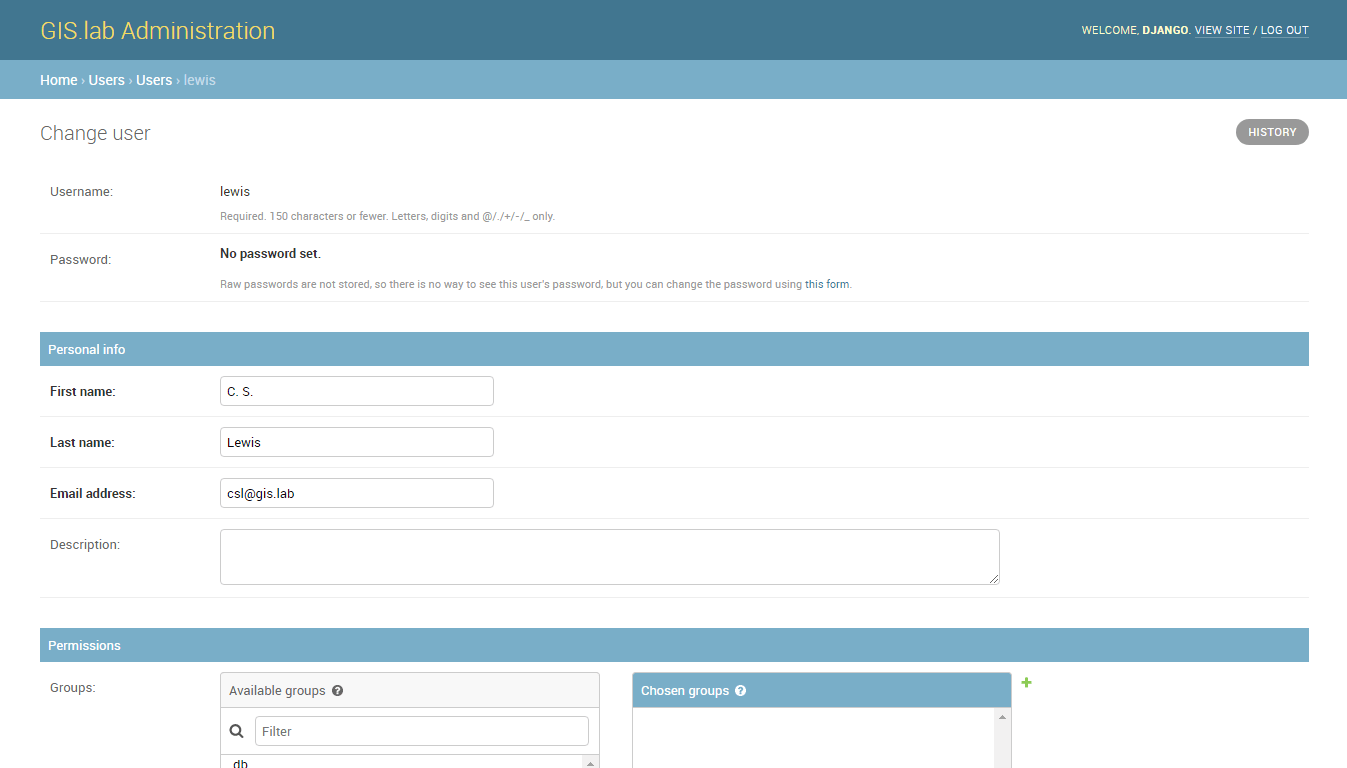
\includegraphics[width=430pt]{./prilohy/guide-admin-changeuser01.png}
    \caption[Admin console - user details 1/2]{Admin console - user details 1/2 (zdroj:
	\href{}{Tereza Kulovaná})}
	\label{fig:guide-admin-changeuser01}
\end{figure}

\begin{figure}[H] \centering
    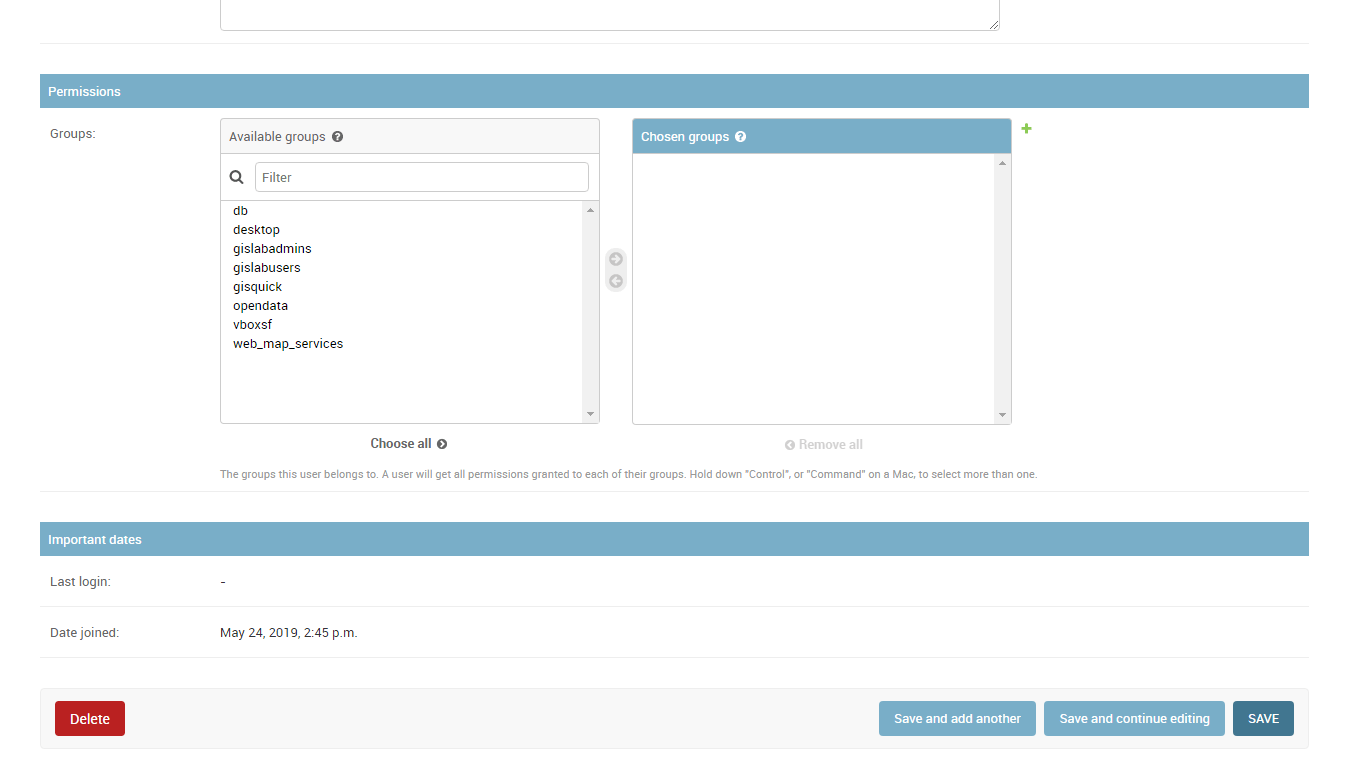
\includegraphics[width=430pt]{./prilohy/guide-admin-changeuser02.png}
    \caption[Admin console - user details 2/2]{Admin console - user details 2/2 (zdroj:
	\href{}{Tereza Kulovaná})}
	\label{fig:guide-admin-changeuser02}
\end{figure}

\newpage
Write new password twice for verification and push the \textsf{CHANGE}
button. In case of a successful change, user's credentials are
updated.
\begin{figure}[H] \centering
    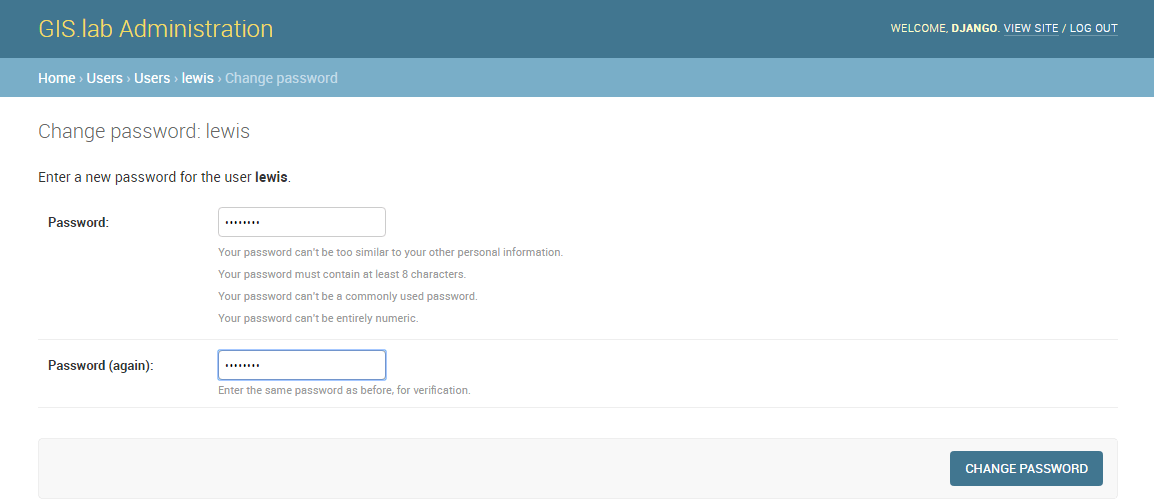
\includegraphics[width=430pt]{./prilohy/guide-admin-password.png}
    \caption[Admin console - change password]{Admin console - change password (zdroj:
	\href{}{Tereza Kulovaná})}
	\label{fig:guide-admin-password}
\end{figure}

\textit{Username, first name, last name, email address and password}
are mandatory fields for successful registration, \textit{description}
is optional. For creating new user push the \textsf{SAVE} button. If
the form is not valid, the error, with information of what went wrong,
is displayed. In case of a successful validation, you are redirected
to page with users list.
\begin{figure}[H] \centering
    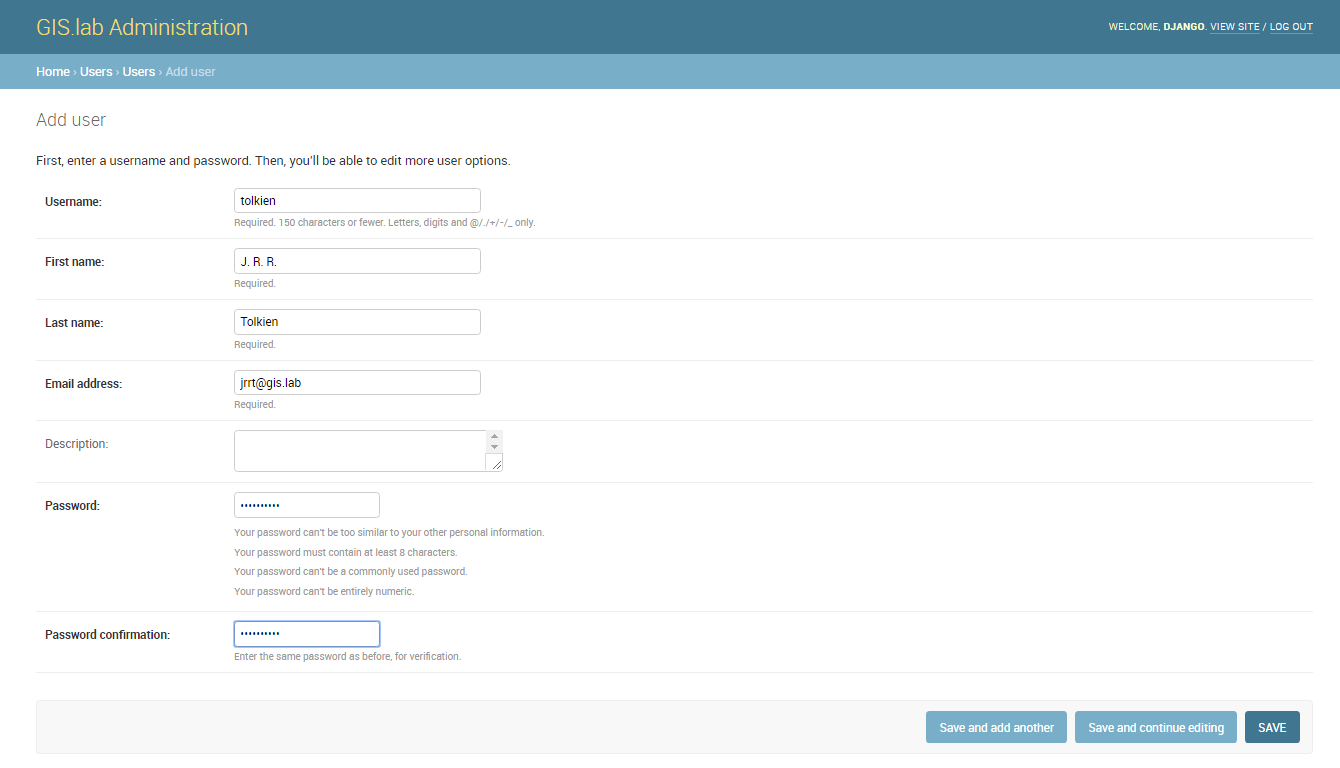
\includegraphics[width=430pt]{./prilohy/guide-admin-user-add.png}
    \caption[Admin console - create new user]{Admin console - create new user (zdroj:
	\href{}{Tereza Kulovaná})}
	\label{fig:guide-admin-user-add}
\end{figure}

Group list displays names of all groups (roles) in database. New group
can be added by \textsf{ADD GROUP} button in the upper right
corner. You can delete group by clicking on its name.
\begin{figure}[H] \centering
    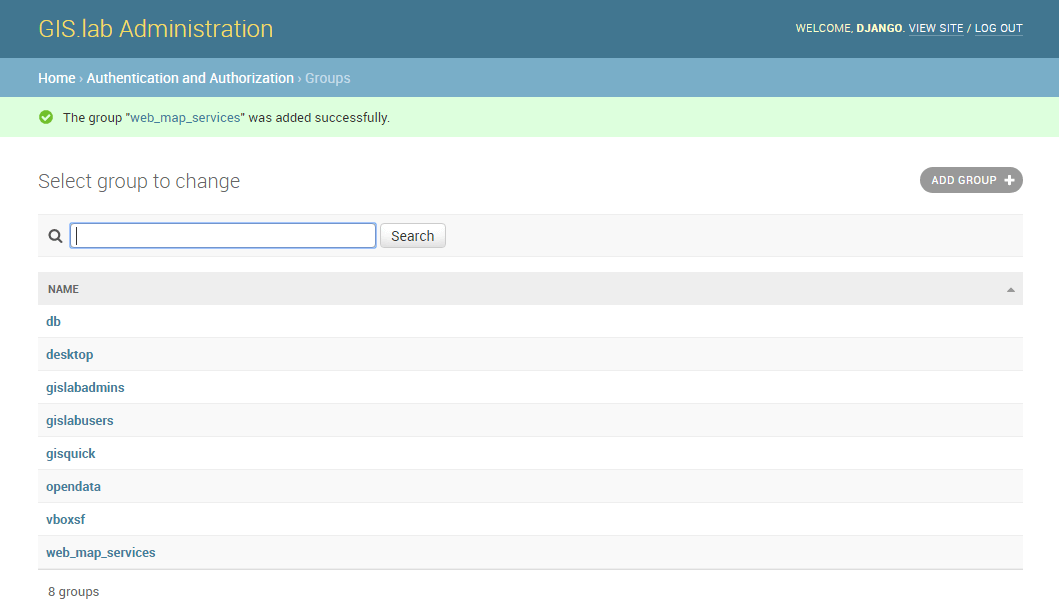
\includegraphics[width=430pt]{./prilohy/guide-admin-groups.png}
    \caption[Admin console - groups]{Admin console - groups (zdroj:
	\href{}{Tereza Kulovaná})}
	\label{fig:guide-admin-groups}
\end{figure}

On group details page you can delete group from database by pushing
\textsf{Delete} button in the bottom left corner. The decision has to
be confirmed.
\begin{figure}[H] \centering
    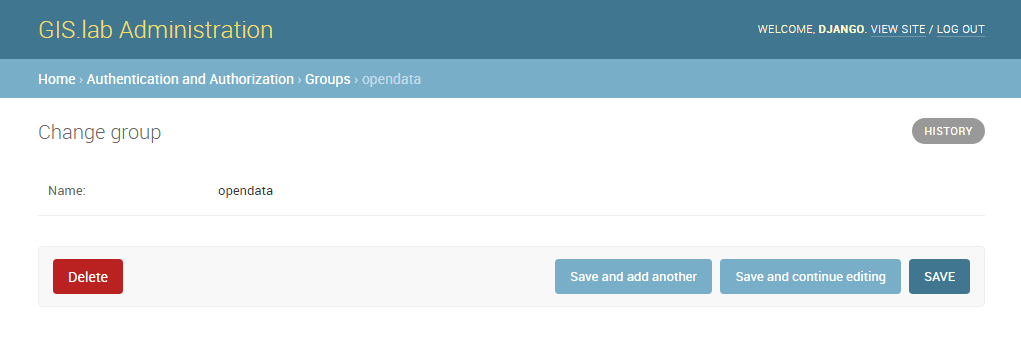
\includegraphics[width=430pt]{./prilohy/guide-admin-group-change.png}
    \caption[Admin console - group details]{Admin console - group details (zdroj:
	\href{}{Tereza Kulovaná})}
	\label{fig:guide-admin-group-change}
\end{figure}

\newpage
Group object has only one atribute, \textit{name}. For creating new
group push the \textsf{SAVE} button. If the group already exists, the
error is displayed. In case of a successful validation, you are
redirected to the page with list of groups.
\begin{figure}[H] \centering
    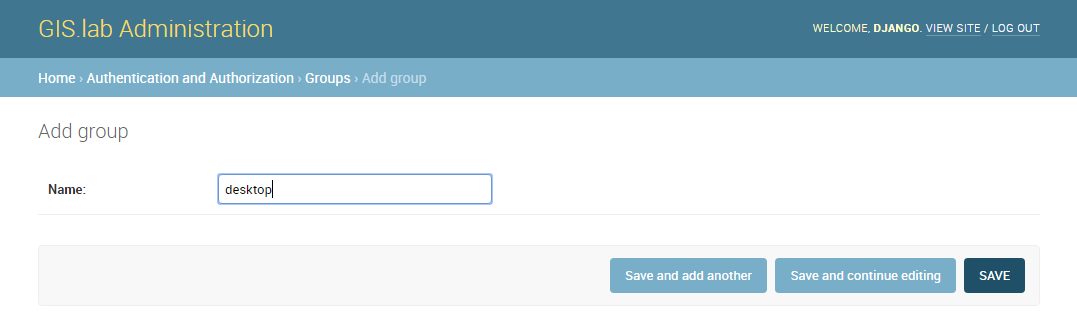
\includegraphics[width=430pt]{./prilohy/guide-admin-group-add.png}
    \caption[Admin console - create new group]{Admin console - create new group (zdroj:
	\href{}{Tereza Kulovaná})}
	\label{fig:guide-admin-group-add}
\end{figure}

Logout is available by \textsf{LOG OUT} link in the upper right
corner. Link \textsf{VIEW SITE} will redirect you to user console.

\chapter{Obsah CD}
\label{cd}


\setlength{\unitlength}{.5mm}
\begin{picture}(250, 220)

  \put(  0, 212){\textbf{.}}

  \put(  1, 200){\line(0, 1){5}}
  \put(  1, 200){\line(1, 0){10} {\textbf{ assignment}}}
  \put(150, 200){ zadání práce}  

  \put(  1,  190){\line(0, 1){10}}
  \put(  1,  190){\line(1, 0){10} {\textbf{ src}}}
  \put(150,  190){ zdrojový kód}                     
          
  \put(  1,  180){\line(0, 1){10}}
  \put(  1,  180){\line(1, 0){10} {\textbf{ text}}}
  \put(150,  180){ text práce ve formátu PDF}
  
\end{picture}
